\documentclass{beamer}
\usepackage{amsmath,amsfonts,amsthm,amstext,amssymb, xcolor, tikz, pgf}

% ----------------------------------------------------------
% Theme Setup

% Use Metropolis Theme
\usetheme[numbering=fraction]{metropolis}
\setbeamertemplate{blocks}[rounded][shadow=false]
\makeatletter
\setlength{\metropolis@titleseparator@linewidth}{1pt}
\makeatother

% Define Colors
\definecolor{chargerblue}{HTML}{002764}
\definecolor{chargerred}{HTML}{e02034}
\definecolor{bggray}{HTML}{d0d3d4}

% Set Colors
\setbeamercolor{title}{fg=chargerblue}
\setbeamercolor{background canvas}{bg=white}
\setbeamercolor{title separator}{fg=chargerred}
\setbeamercolor{structure}{fg=chargerblue}
\setbeamercolor{frametitle}{fg=white, bg=chargerblue}
\setbeamercolor*{normal text}{fg=chargerblue}
\setbeamercolor*{block body}{bg=bggray}
\setbeamercolor*{block title}{bg=chargerblue, fg=white}
% ----------------------------------------------------------

% ----------------------------------------------------------
% Custom Definitions, Commands, Environments, etc.

% Sets of numbers
\def\R{\mathbb{R}} % The reals
\def\N{\mathbb{N}} % The naturals
\def\Z{\mathbb{Z}} % The integers
\def\Q{\mathbb{Q}} % The rationals

% Blank space
\newcommand{\blank}[1]{\underline{\hspace{#1}}} % Blank space

% Fitted inclusion symbols
\newcommand{\fp}[1]{\left({#1}\right)} % Fitted parentheses around content
\newcommand{\fb}[1]{\left[{#1}\right]} % Fitted brackets
\newcommand{\set}[1]{\left\{{#1}\right\}} % Fitted braces (useful for sets)
\newcommand{\av}[1]{\left|{#1}\right|} % Fitted absolute value bars

% To shortcut
\def\to{\rightarrow}



% Coordinate Plane (Four-Quadrant)
\def\coordplane {
	\begin{tikzpicture}		\draw[step=0.25cm,black,very thin,opacity=0.25] (-2.5cm, -2.5cm) grid (2.5cm, 2.5cm);
		\draw[<->,thick,black] (-2.5cm, 0) -- (2.5cm, 0) node[anchor=north west,pos=0.94,font=\scriptsize]{$x$};
		\draw[<->,thick,black] (0,-2.5cm) -- (0, 2.5cm) node[anchor=south east,font=\scriptsize,pos=0.94]{$y$};
	\end{tikzpicture}
}

% Coordinate Plane (One-Quadrant)
\def\onequad {
	\begin{tikzpicture}
		\draw[step=0.25cm, black, very thin, opacity=0.25] (0,0) grid (7.5cm,5cm);
		\draw[->, thick, black] (0,0) -- (7.5cm, 0) node[anchor=north west,font=\scriptsize,pos=0.94]{$x$};
		\draw[->, black, thick] (0,0) -- (0,5cm) node[anchor=south east,font=\scriptsize,pos=0.94]{$y$};
	\end{tikzpicture}
}
% ----------------------------------------------------------

% ----------------------------------------------------------
% Presentation Information 
\title[3.1 and 3.2]{Quadratic Equations and Models; Polynomials of Higher Degree}
\subtitle{Sections 3.1 and 3.2}
\author{Jacob Ayers}
\institute{Lesson \#11}
\date{MAT 130}
% ----------------------------------------------------------

\begin{document}

% Slide 1 (Title Slide)
\begin{frame}
\titlepage
\end{frame}

% Slide 2 (Objectives)
\begin{frame}[t]{Objectives}
\begin{itemize}
	\item Analyze graphs of quadratic functions
	\item Find minimum and maximum values of quadratic functions
	\item Determine end behaviors of polynomial functions using Leading Coefficient Test
	\item Find real zeros of polynomial functions and use them as sketching aids
	\item Use the Intermediate Value Theorem to help locate real zeros of polynomial functions
\end{itemize}
\end{frame}

\begin{frame}[t]{Key Definitions}
\begin{block}{Definition}
Let $n \geq 0 \in \Z$ and let $a_n,a_{n-1},\dots,a_2,a_1,a_0 \in \R$ with $a_n \neq 0$. The function \vspace{-8pt} $$f(x) = a_n x^n + a_{n-1} x^{n-a} + \cdots + a_2 x^2 + a_1 x + a_0$$ is a \textit{polynomial function of $x$ with degree $n$}.
\end{block}

\pause

\begin{block}{Definition}
Let $a,b,c\in\R$ with $a\neq 0$. The function \vspace{-8pt} $$f(x) = ax^2 + bx + c$$ is a \textit{quadratic function}.
\end{block}
\end{frame}

\begin{frame}[t]{Graphs of Quadratic Functions}
The graph of a quadratic function is called a \textit{parabola}. Parabolas are ``U"-shaped.

\pause

The value of $a$ determines which direction the parabola opens. If $a > 0$, then the parabola will open upward; if $a < 0$, then the parabola will open downward.

\pause

All parabolas have what is called a \textit{line of symmetry}.
\end{frame}

\begin{frame}{Graphs of Quadratic Functions}
\begin{columns}
\begin{column}{0.5\textwidth}
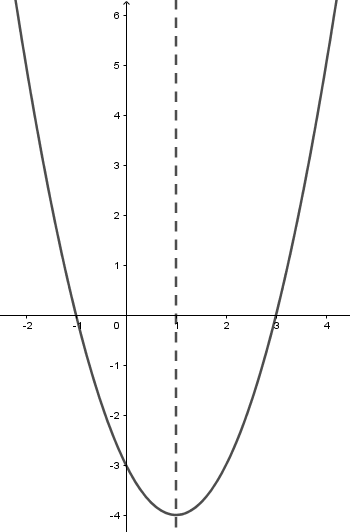
\includegraphics[width=0.75\textwidth]{Quad1.png}
\end{column}
\begin{column}{0.5\textwidth}
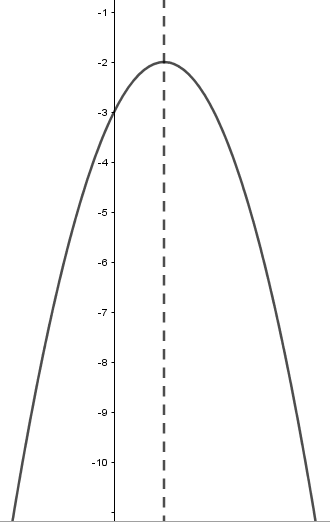
\includegraphics[width=0.75\textwidth]{Quad2.png}
\end{column}
\end{columns}
\end{frame}

\begin{frame}[t]{Minimum and Maximum Values}
We often need to find the minimum or maximum value of a quadratic function in applications.

\pause Looking at the graphs on the previous slide, we can see that a parabola will have a minimum when $a > 0$ and a maximum if $a < 0$.

\pause

That minimum or maximum value is called the \textit{vertex} of the parabola, and it has the coordinates $$\fp{-\dfrac{b}{2a}, f\fp{-\dfrac{b}{2a}}}$$
\pause
We say that $f$ has a \textit{minimum/maximum} at $x=-\dfrac{b}{2a}$ and the \textit{minimum/maximum value} is $f\fp{-\dfrac{b}{2a}}$.
\end{frame}

\begin{frame}[t]{Minimum and Maximum Values}
The path of a baseball after being hit is modeled by $f(x) = -0.007x^2 + x + 4$, where $f(x)$ is the horizontal distance from home plate (in feet). Find the maximum height of the baseball.

\onslide<2->{We can find the maximum height of the ball by evaluating $f\fp{-\dfrac{b}{2a}}$.}

\onslide<3->{$-\dfrac{b}{2a} = -\dfrac{1}{2(-0.007)} \approx 71.4286$ (Note: store the exact value as a variable in your calculator)}
\end{frame}

\begin{frame}[t]{Minimum and Maximum Values}
$f(x) = -0.007x^2 + x + 4$
\begin{flalign*}
\onslide<2->{f\fp{-\dfrac{b}{2a}} &= f(71.4286) & \\}
\onslide<3->{&= -0.007(71.4286)^2 + 71.4286 + 4 & \\}
\onslide<4->{&\approx 39.71}
\end{flalign*}
\onslide<5>{The ball will reach a maximum height of about 39.71 ft. This maximum height will be reached when the ball is about 71.43 feet away from home plate.}
\end{frame}

\begin{frame}[t]{Graphs of Polynomial Functions}
Key features of polynomial graphs: \begin{itemize}
\item Continuous (no breaks, holes, or gaps)
\item Only smooth, rounded turns
\end{itemize}

\pause

Graphing polynomials of a degree higher than 2 is more involved than what we've graphed before. The goal isn't to be perfect when we graph by hand; we just want a reasonably accurate sketch. If perfection is required, we'll use technology.
\end{frame}

\begin{frame}[t]{The Leading Coefficient Test}
The \textit{Leading Coefficient Test} will tell us about the \textit{end behavior} of a polynomial function. \pause The end behavior refers to what the function is doing as it approaches $-\infty$ and $+\infty$.
\end{frame}

\begin{frame}[t]{The Leading Coefficient Test}
\begin{block}{The Leading Coefficient Test}
Suppose we have a polynomial function $f(x) = a_nx^n + a_{n-1}x^{n-1} + \cdots + a_2x^2 + a_1x + a_0$. We can determine the end behavior of the function by looking at the degree and the leading coefficient. \vspace{12pt}

If $n$ is odd: \begin{itemize}
\item If $a_n > 0$, then $f(x) \to -\infty$ as $x \to -\infty$ and $f(x) \to \infty$ as $x \to \infty$
\item If $a_n < 0$, then $f(x) \to \infty$ as $x \to -\infty$ and $f(x) \to -\infty$ as $x \to \infty$
\end{itemize}
\end{block}
\end{frame}

\begin{frame}[t]{The Leading Coefficient Test}
\begin{block}{The Leading Coefficient Test}
Suppose we have a polynomial function $f(x) = a_nx^n + a_{n-1}x^{n-1} + \cdots + a_2x^2 + a_1x + a_0$. We can determine the end behavior of the function by looking at the degree and the leading coefficient. \vspace{12pt}

If $n$ is even: \begin{itemize}
\item If $a_n > 0$, then $f(x) \to \infty$ as $x \to -\infty$ and $f(x) \to \infty$ as $x \to \infty$
\item If $a_n < 0$, then $f(x) \to -\infty$ as $x \to -\infty$ and $f(x) \to -\infty$ as $x \to \infty$
\end{itemize}
\end{block}
\end{frame}

\begin{frame}[t]{Describing End Behavior Using LCT}
Use the Leading Coefficient Test to determine the end behavior of $f(x) = 5x^3 - 4x^3 + 3x^3 - 2x^2 + x - 1$.

\pause

First, identify the degree and the leading coefficient: Degree is $3$, Leading Coefficient is $5$.

\pause Since $n$ is odd and $a_n > 0$, we conclude that the graph approaches $-\infty$ as $x$ goes to $-\infty$ and the graph approaches $\infty$ as $x$ goes to $\infty$.

\pause

We can confirm this visually.
\end{frame}

\begin{frame}[t]{Describing End Behavior Using LCT}
Use the Leading Coefficient Test to determine the end behavior of $f(x) = -8x^2 + 51x - 18$.

\pause

First, identify the degree and the leading coefficient: Degree is $2$, Leading Coefficient is $-8$.

\pause

Since $n$ is even and $a_n < 0$, we conclude that the graph approaches $-\infty$ as $x$ goes to $-\infty$ and the graph approaches $-\infty$ as $x$ goes to $\infty$.

\pause

We can confirm this visually.
\end{frame}

\begin{frame}[t]{Real Zeros}
A function of degree $n$ has at most $n$ real zeros and at most $n - 1$ turning points.

\begin{block}{Real Zeros of Polynomial Functions}
When $f$ is a polynomial function and $a$ is a real number, the statements listed below are equivalent. \begin{enumerate}
\item $x = a$ is a zero of $f$.
\item $x = a$ is a solution of the equation $f(x) = 0$.
\item $(x-a)$ is a factor of $f(x)$.
\item $(a, 0)$ is an $x$-intercept of the graph of $f$.
\end{enumerate}
\end{block}
\end{frame}

\begin{frame}[t]{Real Zeros}
Find all real zeros of $f(x) = x^3 - 12x^2 + 36x$. Then determine the maximum number of turning points of the graph of the function.

\pause

We can find the real zeros by factoring: \\
$x^3 - 12x^2 + 36x = x\fp{x^2 - 12x + 36} = x\fp{x-6}^2$

\pause

Therefore, the real zeros of the function are $x = 0$ and $x = 6$.

\pause

Since $n = 3$, there are a maximum of $3 - 1 = 2$ turning points in the graph of $f(x)$.
\end{frame}

\begin{frame}[t]{Repeated Zeros}
In the previous example, we found that $f(x) = x^3 - 12x^2 + 36x$ could be factored to $x(x-6)^2$. In this case, $x = 6$ is called a \textit{repeated zero}.

\begin{block}{Repeated Zeros}
A factor $(x - a)^k, k > 1$, yields a \textit{repeated zero} $x = a$ of \textit{multiplicity} $k$. \begin{itemize}
\item If $k$ is odd, then the graph will \textit{cross} the line at $x = a$.
\item If $k$ is even, then the graph will \textit{touch} the line at $x = a$.
\end{itemize}
\end{block}
\end{frame}

\begin{frame}[t]{Putting It All Together}
If we put together everything we've learned, we can do a pretty good job graphing any polynomial function. 

\pause

To sketch the graph of a polynomial function: \begin{enumerate}[1)]
\item Use LCT to determine end behavior
\item Find and plot any real zeros, and note their multiplicity
\item Plot additional points as needed
\item Connect your points with smooth curves
\end{enumerate}
\end{frame}

\begin{frame}[t]{Sketching Graphs of Polynomial Functions}
Sketch the graph of $f(x) = 2x^3 - 6x^2$.

\pause

1) Use LCT: $n = 3$ (odd), $a_n = 2 > 0$ \\
Conclusion: $f(x) \to -\infty$ as $x\to -\infty$ and $f(x) \to \infty$ as $x \to \infty$

\pause

2) Real Zeros: $2x^3 - 6x^2 = 2x^2\fp{x - 3}$ \\
Conclusion: Real zeroes at $x = 0$ (touch) and $x = 3$ (cross)

\pause

Additional Points (gathered using table tool on calculator): \\
\begin{tabular}{c|c}
$x$ & $f(x)$ \\ \hline
$-2$ & $-40$ \\
$-1$ & $-8$ \\
$1$ & $-4$ \\
$2$ & $-8$ \\
$4$ & $32$
\end{tabular}
\end{frame}

\begin{frame}[t]{Sketching Graphs of Polynomial Functions}
\coordplane
\end{frame}

\begin{frame}[t]{Sketching Graphs of Polynomial Functions}
Sketch the graph of $f(x) = -\dfrac14 x^4 + \dfrac32 x^3 - \dfrac94 x^2$.

\pause

1) LCT: $n = 4$ (even), $a_2 = -\dfrac14 < 0$ \\
Conclusion: Conclusion: $f(x) \to -\infty$ as $x\to -\infty$ and $f(x) \to -\infty$ as $x \to \infty$

\pause

2) Real zeros: \begin{flalign*}
-\dfrac14 x^4 + \dfrac32 x^3 - \dfrac94 x^2 &= -\dfrac14 x^4 + \dfrac64 x^3 - \dfrac94 x^2 & \\
&= -\dfrac14 x^2\fp{x^2 - 6x + 9} & \\
&= -\dfrac14 x^2\fp{x-3}^2
\end{flalign*}
Conclusion: Real zeros at $x = 0$ (touch) and $x = 3$ (touch).
\end{frame}

\begin{frame}{•}
\begin{columns}
\begin{column}{0.5\textwidth}
3) Additional points: \\
\begin{tabular}{c|c}
$x$ & $f(x)$ \\ \hline
$-2$ & $-25$ \\
$-1$ & $-4$ \\
$1$ & $-1$ \\
$2$ & $-2$ \\
$4$ & $-4$ \\
$5$ & $-25$
\end{tabular}
\end{column}
\begin{column}{0.5\textwidth}
\coordplane
\end{column}
\end{columns}
\end{frame}

\begin{frame}[t]{The Intermediate Value Theorem}
\begin{block}{The Intermediate Value Theorem}
Let $a,b \in \R$ such that $a < b$. If $f$ is a polynomial function such that $f(a) \neq f(b)$, then, in the interval $[a,b]$, $f$ takes on every value between $f(a)$ and $f(b)$
\end{block}

\pause

You'll see a lot more of the Intermediate Value Theorem in Calculus.

For now, we'll apply it to approximate real zeros of polynomials.

\pause

The idea is this: Whenever we find $x_1$ for which $f(x) < 0$ and $x_2$ for which $f(x) > 0$, there must be a real zero between $x_1$ and $x_2$. Then we keep narrowing the range. 
\end{frame}

\begin{frame}[t]{The Intermediate Value Theorem}
Use the Intermediate Value Theorem to approximate the real zero of $f(x) = x^3 - 3x^2 - 2$.

I'll be doing this using a TI-84, but will post videos showing you how to do it on other utilities.

\pause

There is a real zero between $x = 3.19$ and $x = 3.20$.
\end{frame}

\begin{frame}[t]{Next Steps}
\begin{itemize}
\item Post questions in Lesson 11 forum, if you have any
\item Read 3.3 and 3.4
\item Watch Video Lessons \#12 and \#13
\item Complete Assignment \#6
\end{itemize}
\end{frame}

\end{document}